\part{Analyse de l'existant}


\section{Fonctionnement de l'application Royal}

\subsection{Introduction}
Nous n'avions pas d'existant imposé à proprement parlé, cependant nous avons été guidé vers Royal, un projet existant réalisé par des étudiants du département informatique de l'an passé.
Il apparait être une des solutions actuelles la plus en accord avec la demande du client, à savoir, de manière générale : « la gestion d'une bédéthèque ».

De ce fait, cet article traitera du fonctionnement de Royal.
C'est une application 
libre \footnote{Selon les termes de la GNU Lesser General Public License}
issue d'une amélioration de \emph{Birdy}, une autre application libre de gestion de livres.

\subsection{Aspect fonctionnel de Royal}
Royal permet la saisie d'informations sur une bande déssinée, tel que son titre, son auteur, son image de couverture (recherchée sur internet), sa date de parution, etc..
Il permet d'obtenir une liste de l'ensemble des \emph{BDs}, que l'on peut trier selon divers critères et réorganiser selon des collections de \emph{BDs}.
Royal permet l'enregistrement de \emph{BDs}, mais aussi d'informations concernant les auteurs ou encore les collections.

On peut aussi importer un ensemble de \emph{BD} à partir d'une base de données existante.
De plus, Royal intègre un système multi-lingues concernant son interface utilisateur, ainsi que d'une bibliothèque d'aide d'utilisation.

Après cette brève description de Royal, on peut observer que son utilisation permet déjà de répondre à plusieurs fonctionnalités décrites auparavant. Cela permettra de se concentrer sur les fonctions manquantes ici que sur l'amélioration de l'existant.

\subsection{Aspect technique de Royal}
Royal est développé en Java et utilise la bibliothèque \emph{Swing} pour son environnement graphique. 
Le projet à été développé sous Linux, mais reste néanmoins éxécutable sous d'autres systèmes d'exploitations comme Windows 7 par exemple, avec plus ou moins de succès. 
L'ensemble des données stockées est réalisé via \emph{Hibernate}, c'est un framework gérant la persistance des objets en base de données. 
C'est un outil lourd et complexe mais très puissant que nous allons ré-utiliser étant donné son existence sous Royal, qui permet un transfert simplifié entre objets java et base de données.

\subsection{Analyse de la base de données}

Comme nous pouvons l'observer, le MCD existant traite un certains nombres d'information néccéssaire pour l'enregistrement des information de notre livre.
Les tables Emprunteur et Location ne sont actuellement inutilisé dans Royal mais pourrait nous permettre l'enregistrement de la date de retour.
Néanmoin des tables devrons lui étre ajouté afin de rendre possible la sauvegarde d'information concernant les bibliotèques.. 


\begin{figure}[hp]
 \centering
 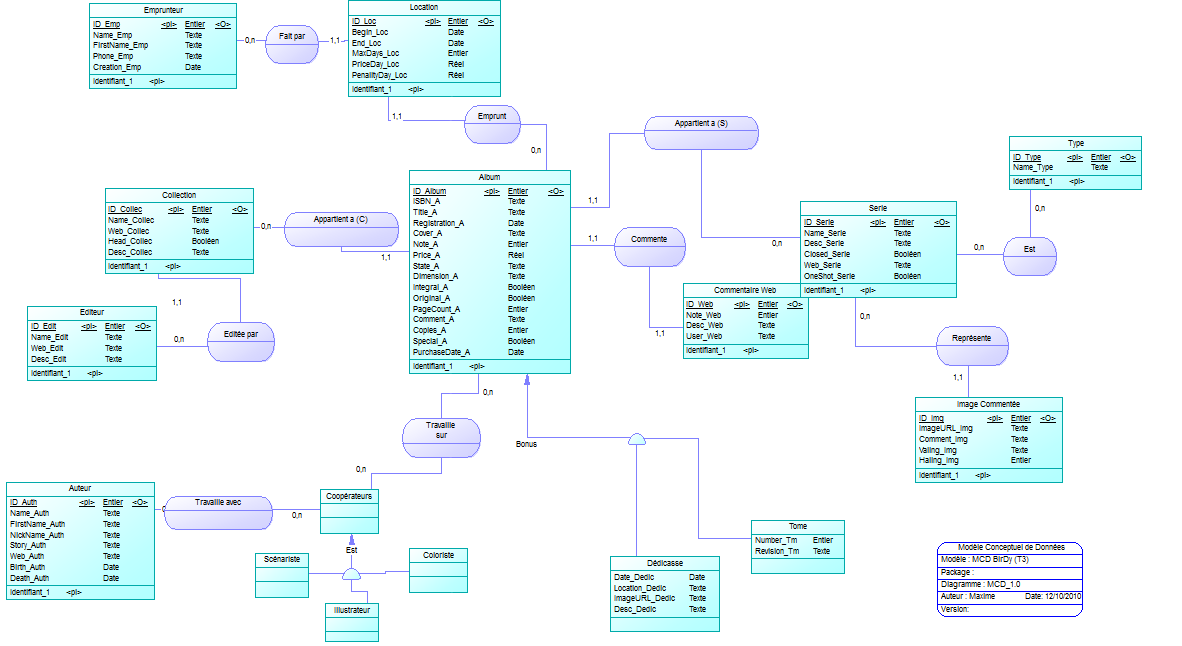
\includegraphics[height=24cm]{../img/MCD_Royal.png}
 % MCD_Royal.png: 646x1182 pixel, 96dpi, 17.09x31.28 cm, bb=0 0 485 887
\end{figure}

